\documentclass[conference]{IEEEtran}

\usepackage{cite}
\usepackage{amsmath,amssymb}
\usepackage{algorithm}
\usepackage{algpseudocode}
\usepackage{algpseudocode}
\usepackage{graphicx}
\usepackage{textcomp}
\usepackage{xcolor}
\usepackage{cleveref}
\usepackage{pdfpages}


\def\BibTeX{{\rm B\kern-.05em{\sc i\kern-.025em b}\kern-.08em
    T\kern-.1667em\lower.7ex\hbox{E}\kern-.125emX}}

\begin{document}

\title{ECM2427: Literature Review on SAT Solvers}
\author{\IEEEauthorblockN{Anonymised Author}}

\onecolumn

\section*{AI Declaration}
AI-supported/AI-integrated use is permitted in this assessment. I acknowledge the following uses of GenAI tools in this assessment:
\begin{itemize}
    \item I have used GenAI tools to assist with research or gathering information.
    \item I have used GenAI tools to help me understand key theories and concepts.
    \item I have used GenAI tools to give me feedback on a draft.
\end{itemize}
I declare that I have referenced use of GenAI outputs within my assessment in line with the University referencing guidelines.

\newpage
\twocolumn

\maketitle

\section{Introduction}
Satisfiability (SAT) solvers are algorithms designed to determine the satisfiability of boolean formulae, a problem that is central to both theoretical and practical computer science. SAT was one of the first problems proven to be NP-complete, and as such, it has been the subject of extensive research \cite{gong2017survey}\cite{cook2023complexity}.

A boolean formula is a logical expression that consists of propositional variables \(x_1, x_2, \ldots, x_n\) and the boolean operations AND (\(\land\)), OR (\(\lor\)), and NOT (\(\neg\)). A formula is said to be satisfiable if there exists an assignment of truth values to the variables that makes the formula true. SAT solvers are algorithms that determine whether such an assignment exists, and can normally produce one if it does \cite{gong2017survey}.

Consider the small formula:
\begin{equation}
    (x_1 \lor x_2) \land (\neg x_1 \lor x_3) \land (\neg x_2 \lor \neg x_3)
    \label{eq:small_example}
\end{equation}
This formula is in conjunctive normal form (CNF), a standard representation for boolean formulae, where each clause is a disjunction of literals, and the formula is a conjunction of clauses \cite{gelder2011generalized}. \Cref{eq:small_example} has only three variables and three clauses, and so it is easy to manually determine that \(x_1 = \text{true}\), \(x_2 = \text{false}\), and \(x_3 = \text{true}\) is a satisfying assignment.

The terminology `\(k\)-SAT' refers to the problem of determining the satisfiability of a boolean formula in CNF where each clause has at most \(k\) literals.

Because SAT is an NP-complete problem, all other NP problems can be reduced to SAT in polynomial time. This makes SAT solvers a powerful tool for solving a wide range of problems in computer science, including hardware and software verification, planning, scheduling, and many others.

% TODO Ensure this is still correct.
This literature review examines the evolution of SAT solvers since their inception in the 1960s. The scope of the review include works that laid the foundations of SAT solving, subsequent enhancements such as conflict-driven clause learning (CDCL), and contemporary enhancements including parallel approaches and restart heuristics. The empirical performance of these methods in industry is also considered.

Sources were selected based on their impact and relevance, with peer-reviewed journal articles and conference papers being prioritised. The \emph{Theory and Applications of Satisfiability Testing} conference series was a key source of information, as it is the premier conference for SAT solvers that has been running for a number of years.

\section{Review}
My review structure is thematic.

\subsection{Foundations of SAT Solving}
Mainstream SAT solvers come in two varieties: complete and incomplete. An algorithm is considered incomplete if it is not guaranteed to find a solution, whilst a complete solver will search the entire space and so is able to prove that a formula is unsat \cite{gong2017survey}.

The first systematic approach to SAT solving was introduced by Davis and Putnam in 1960, intended to solve the problem of validity in propositional logic. Their method improved on previous methods, allowing a formula that took 21 minutes to solve on an IBM 704 machine to be solved by hand in 30 \cite{martin1960computing}. Their algorithm was furthered by Longemann and Loveland with the addition of backtracking to produce what is now known as DPLL, the basis for many modern SAT solvers \cite{gong2017survey}.

\subsubsection{DPLL}
The DPLL algorithm uses the eager application of two basic rules: unit propogration and pure literal elimination.

A unit clause is one that contains a single unassigned literal, which therefore must be true. This implies that all other clauses containing the literal will be satisfied (recall that in CNF, each clause is a disjunction of literals), and so can be removed from the formula.

Pure literals are those that appear with only one polarity in the formula. Assigning such a literal so that it satisfies all clauses that contains it allows all of these clauses to be removed.

If neither of these rules can be applied, the algorithm selects a variable and assigns it a truth value, then recursively calls itself with the updated formula. If the formula is unsatisfiable, the algorithm backtracks and tries the opposite truth value for the variable. This process is repeated until a satisfying assignment is found or all variables have been assigned \cite{marques1999impact}.

\subsubsection{Incomplete Solvers}
An example of an incomplete solver is GSAT. GSAT uses a greedy hill-climbing algorithm to search for a satisfying assignment, starting from a random assignment of variables. The algorithm then flips the variable assignment that leads to the largest increase in the number of satisfied clauses, repeating until a satisfying assignment is found or a limit is reached. If no satisfying assignment is found, this process can be repeated from another random assignment \cite{gent1993empirical}.

These incomplete solvers are able to solve larger and more difficult problems than complete solvers, although at the disadvantage of not being able to prove unsatisfiability \cite{gent1993empirical}.

A study of GSAT on random 3-SAT problems found that the algorithm tends to plateau after a certain number of steps, with the first few variable flips leading to a large number of satisfied clauses, but later flips having little effect.

\subsection{Conflict-Driven Clause Learning}
Conflict-Driven Clause Learning (CDCL) was introduced by Marques-Silva and Sakallah in 1999 with their GRASP solver \cite{marques1999grasp}. CDCL solvers improve significantly on DPLL solvers, allowing complete solvers to be used in practical applications \cite{marques2008handbook}.

CDCL solvers use a backtracking search, similar to DPLL, but add the ability to learn new clauses from conflicts. When a variable \(x_i\) is implied by unit propogation the implied variable is assigned a \emph{antecedent} \(\alpha(x_i)\) equal to the clause that caused the assignment \cite{marques2008handbook}\cite{gelder2011generalized}.

From these antecedents, a graph can be constructed that represents the implication relationships between variables. This graph is called an \emph{implication graph}. Each node in the graph represents a variable assignment, with the addition of a special \emph{conflict node} \(\kappa\). If \(\alpha(x_i) = \omega\), then there is a directed edge from every variable in the clause \(\omega\), except \(x_i\), to \(x_i\). If unit propogration leads to an unsatisfied clause \(\omega_j\), then \(\omega_j\) is set as the antecedent of \(\kappa\) and a conflict resolution procedure is taken \cite{marques2008handbook}.

Conflict resolution in a CDCL solver has two parts: conflict analysis to identify the clause to be learnt, and backtracking to a previous decision level identified by the conflict analysis.

The efficiency of CDCL solvers can be improved with \emph{clause minimisation}, which aims to remove redundant literals from the learnt clause \cite{katebi2011empirical}.

\subsection{Enhancements}
\subsubsection{Restarts}
In 1997, Gomes et al. discovered through experimentation on combinatorial search problems that these searches exhibit a high variability in performance, with some searches taking a long time to find a solution, and others finding a solution quickly even for the same problem. They coined the term `heavy-tailed behaviour' to describe this phenomenon, because of the distribution of search times \cite{gomes1997heavy}. This behaviour is also observed in SAT solvers.

To address this, Gomes et al. introduced a restart strategy that restarts the search after a certain number of conflicts. This strategy was found to improve the performance of the solver, with the number of restarts being a key parameter in the performance of the solver \cite{gomes1997heavy}. Random restarts allow the solver to escape local minima and explore other parts of the search space that may contain a solution or useful conflict information \cite{katebi2011empirical} \cite{moskewicz2001chaff}.

\subsubsection{VSIDS}
The simple DPLL algorithm chooses an arbitrary variable to assign at each step, but it could be assumed that some variables are more important than others in determining the satisfiability of the formula. A number of strategies can been used, with one of the simplest being \emph{dynamic largest individual sum} (DLIS), which assigns the variable that appears in the most clauses \cite{moskewicz2001chaff}.

A more sophisticated heuristic is \emph{variable state independent decaying sum} (VSIDS). This works as follows:
\begin{enumerate}
    \item Each variable assignment is given a counter initialised at zero.
    \item When a clause is added to the formula (either from the input or as a learnt clause), the counter of each literal in the clause is incremented.
    \item When an assignment needs to be made, the literal with the highest counter is chosen. Ties can be broken using heuristics or randomly.
    \item The counters are decayed over time by dividing by some constant.
\end{enumerate}
VSIDS attempts to satisfy recent conflict clauses, as they are likely to be important in determining the satisfiability of the formula. This strategy dramatically increases performance on large problems, with little performance impact on smaller problems \cite{moskewicz2001chaff}.

\subsubsection{Data Structures}
A naive SAT solver would spend a large amount of time searching for unit clauses after each variable assignment. The efficiency of SAT solvers can be improved by using a more efficient method to locate unit clauses. The most common way to do this is to use a data structure called a \emph{watched literal}. This structure `watches' only two literals in each clause. If both are not false (that is, they are either true or unassigned), then the clause is not a unit clause. The clause now only needs to be visited when one of the two watched literals are assigned false. In this case, one of two conditions must now hold \cite{moskewicz2001chaff}:
\begin{enumerate}
    \item The clause is (still) not a unit clause. In this case, the updated literal is no longer watched, and a new unassigned literal is selected to watch.
    \item The clause has become a unit clause. The watched literal that was not assigned false must be the implied literal, and the procedure for an implied clause is followed.
\end{enumerate}
This data structure significantly improves the performance of SAT solvers by reducing the number of memory accesses and so minimises cache-misses, a key bottleneck in SAT solving \cite{moskewicz2001chaff}.

\subsubsection{Effects of Enhancements}
The combination of these enhancements has a significant impact on the performance of SAT solvers, especially for large problems. \Cref{fig:impact_of_enhancements} shows how the runtime of a SAT solver changes as these features are removed, as measured by the time taken to execute some number of instances\footnote{Instances came from a variety of sources and ranged from 50 variables and 159 clauses to 2,270,930 variables and 8,901,845 clauses \cite{katebi2011empirical}.} \cite{katebi2011empirical}.
\begin{figure}
    \centering
    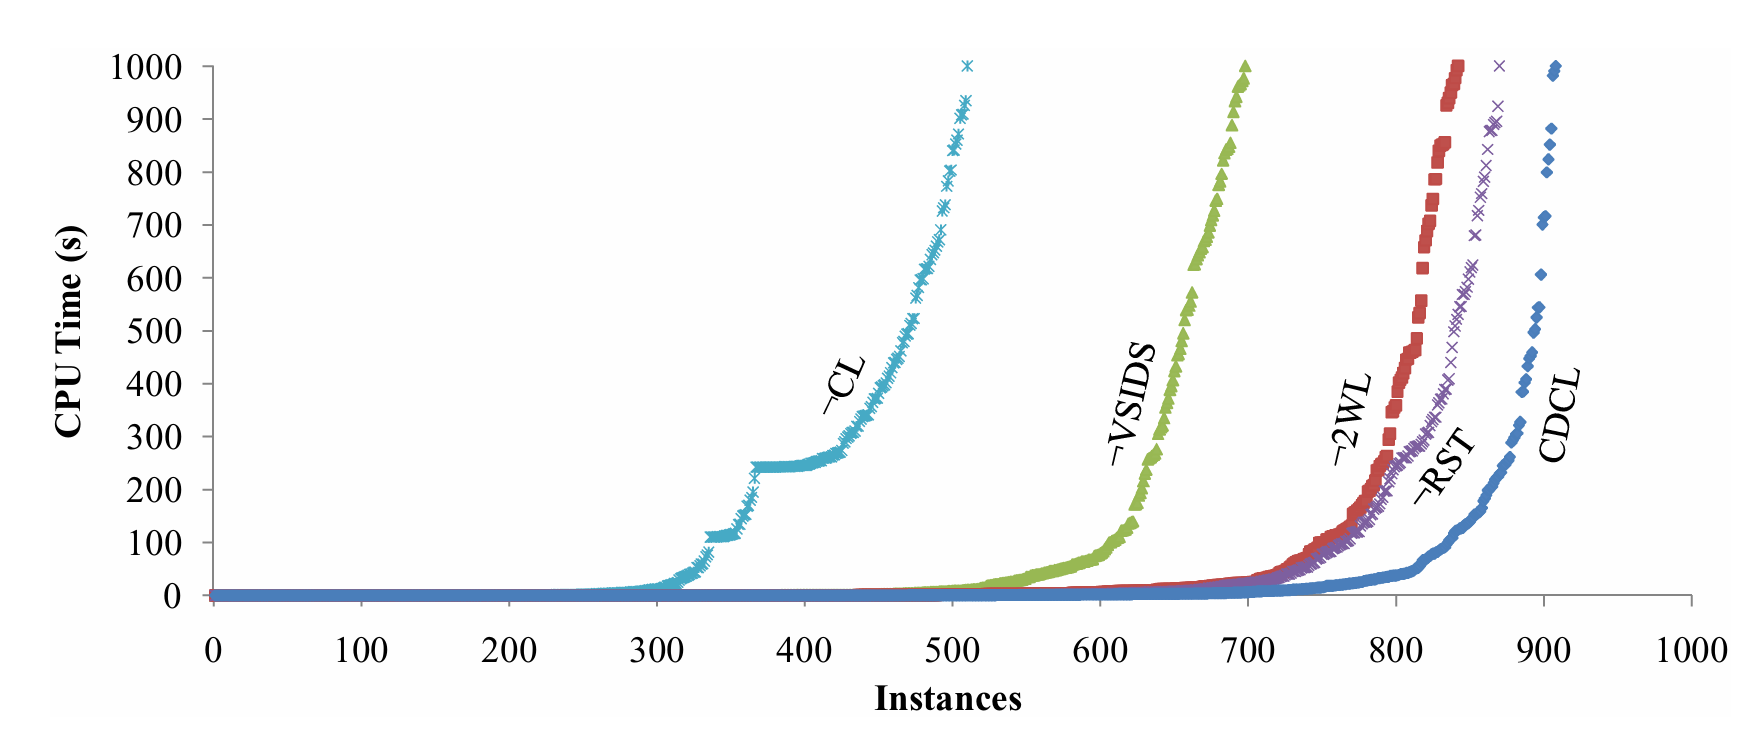
\includegraphics[width=0.45\textwidth]{images/impact_of_enhancements.png}
    \caption{The impact of enhancements on MiniSAT's performance when clause learning (CL), VSIDS, watched literals (2WL), or restarts (RST) are removed. \cite{katebi2011empirical}.}
    \label{fig:impact_of_enhancements}
\end{figure}
Removing clause learning (CL) had a major impact on the performance of the solver, halving the number of instances that could be solved in a given time. Removing VSIDS reduced performance by around a third, showing its significant performance gain over DLIS. Watched literals and restarts had a smaller impact.

\subsection{Practical Applications}
SAT solvers have a wide range of practical applications. The efficiency of current solvers allow them to operate on a large number of clauses, with some solvers able to handle millions of clauses \cite{marques2008handbook}.

\subsubsection{Software Verification}
Model checking is a technique for the verification of systems which automatically produces a witness to the correctness of a system. These methods often work by transforming a program into a boolean formula, which is then passed to a SAT solver to determine the satisfiability of the formula. These methods can verify a range of properties including the reachability of certain states, identify array bounds violations, NULL pointer dereferences, and memory leaks \cite{ivancic2008efficient}.

The predominant method for software verification is \emph{predicate abstraction}, which abstracts the program into a boolean formula that can then be passed to a SAT solver. A simple predicate \(p\) can be a statement such as \(i=0\). In this case a statement such as \texttt{i++}, when executed in a state satisfying \(p\), leads to a state satisfying \(\neg p\). This allows the program to be abstracted into a boolean formula that can be passed to a SAT solver \cite{biere2009handbook}.

\subsubsection{Cryptanalysis of Hash Functions}
Secure hash functions are essential to strong cryptography, and so formal verification of these functions is important. One of the properties that makes a hash function secure is its \emph{collision-resistance}, that is, the difficulty of finding two different inputs \(x\) and \(y\) for which \(H(x) = H(y)\) \cite{mirnov2006applications}.

At their core, hash functions use block ciphers like the Feistel Ladder (used by DES). Algorithms exist to turn such functions into logical circuits, which can then be transformed into a boolean formula and passed to a SAT solver \cite{mirnov2006applications}

In 2006, Mirinov et al. used a SAT solver to find collisions in both the MD4 and MD5 hash functions. Finding a collision for a given message in MD4 could be done in under ten minutes, whilst MD5 required a more convoluted probalistic approach that took a few days on a standard PC.

\section{Conclusion}
This review has traced the evolution of SAT solvers from their foundational roots in DPLL algorithms to the sophisticated, conflict-driven techniques that form modern approaches.

The transition from early exhaustive methods to more refined strategies and their associated enhancements, including restart policies, VSIDS heuristics, and efficient data structures like watched literals, has significantly improved solver performance and scalability.

As SAT solvers become more efficient, their practical applications have also increased. Applications of SAT solving in areas such as software verification and cryptanalysis underscore its pivotal role in modern computer science.

\bibliographystyle{ieeetr}
\bibliography{reference.bib}

\end{document}
